% REV02 Fri 23 Jul 2021 17:19:30 WIB
% REV01 Sun 28 Mar 2021 09:52:23 WIB
% START Fri 26 Mar 2021 17:22:59 WIB

\chapter{ON THE LOOK OUT}

In these times of ours, though concerning the exact year there is no
need to be precise, a boat of dirty and disreputable appearance,
with two figures in it, floated on the Thames, between Southwark
bridge which is of iron, and London Bridge which is of stone, as an
autumn evening was closing in.

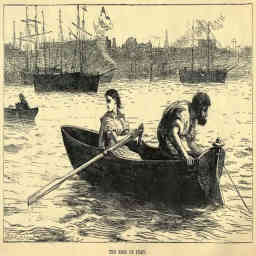
\includegraphics[scale=2.3]{01-01-01}

The figures in this boat were those of a strong man with ragged
grizzled hair and a sun-browned face, and a dark girl of nineteen or
twenty, sufficiently like him to be recognizable as his daughter.
The girl rowed, pulling a pair of sculls very easily; the man, with
the rudder-lines slack in his hands, and his hands loose in his
waistband, kept an eager look out. He had no net, hook, or line,
and he could not be a fisherman; his boat had no cushion for a
sitter, no paint, no inscription, no appliance beyond a rusty
boathook and a coil of rope, and he could not be a waterman; his
boat was too crazy and too small to take in cargo for delivery, and
he could not be a lighterman or river-carrier; there was no clue to
what he looked for, but he looked for something, with a most intent
and searching gaze. The tide, which had turned an hour before,
was running down, and his eyes watched every little race and eddy
in its broad sweep, as the boat made slight head-way against it, or
drove stern foremost before it, according as he directed his
daughter by a movement of his head. She watched his face as
earnestly as he watched the river. But, in the intensity of her look
there was a touch of dread or horror.

